\documentclass[a4paper,10pt]{article}
\usepackage[utf8]{inputenc}
\usepackage[top=0.9cm, bottom=0.8cm, left=1.2cm, right=1.2cm]{geometry}
\usepackage{xcolor}
\usepackage{tabularx}
\usepackage{tcolorbox}
\usepackage{graphicx}
\usepackage{enumitem}
\usepackage{hyperref}
\usepackage{tikz}
\usetikzlibrary{shapes.geometric, arrows, positioning}
\usepackage{helvet}
\renewcommand{\familydefault}{\sfdefault}

% Brand Color Definitions (Claude & Solewise Aesthetic)
\definecolor{soleterracotta}{HTML}{D97757}
\definecolor{soledark}{HTML}{201E1B}
\definecolor{soleivory}{HTML}{FAF9F5}
\definecolor{soleborder}{HTML}{E6E0D6}
\definecolor{solegreen}{HTML}{2E6B4F}
\definecolor{solegray}{HTML}{736E65}

\pagestyle{empty}
\setlength{\parindent}{0pt}
\setlength{\parskip}{2pt}

\hypersetup{
    colorlinks=true,
    linkcolor=soleterracotta,
    urlcolor=soleterracotta
}

\begin{document}

% --- HEADER BLOCK ---
\begin{minipage}[c]{0.70\textwidth}
    {\LARGE \textbf{\color{soledark}SOLEWISE · FOOTWEAR INTELLIGENCE}} \\[2pt]
    {\small \color{soleterracotta} \textbf{Technical Whitepaper: System Genesis, Failure Analysis \& Full-Stack Architecture}}
\end{minipage}
\hfill
\begin{minipage}[c]{0.28\textwidth}
    \raggedleft
    {\footnotesize \textbf{Status:} \color{solegreen} Production Live}\\[1pt]
    {\footnotesize \textbf{Host:} \href{https://sole-wise.onrender.com}{sole-wise.onrender.com}}\\[1pt]
    {\footnotesize \textbf{Stack:} FastAPI + React + PostgreSQL}
\end{minipage}

\vspace{3pt}
{\color{soleterracotta}\hrule height 1.5pt}
\vspace{4pt}

% --- EXECUTIVE SUMMARY ---
\begin{tcolorbox}[colback=soleivory, colframe=soleborder, arc=3pt, boxrule=0.75pt, top=4pt, bottom=4pt, left=8pt, right=8pt]
    \footnotesize
    \textbf{Executive Summary:} \color{soledark}
    Solewise was engineered to replace fragmented, error-prone spreadsheets in footwear manufacturing with an automated, dual-specification technical alternative matrix and batch yield optimizer. This report documents the critical engineering challenges encountered—including ephemeral cloud container data loss, Excel export encoding breakdown, and test fixture database pollution—alongside the architectural solutions deployed across database persistence, client ergonomics, and full-stack cloud infrastructure.
\end{tcolorbox}

\vspace{3pt}

% --- KEY PERFORMANCE METRICS BAR ---
\begin{tabularx}{\textwidth}{@{} *{4}{X} @{}}
    \begin{tcolorbox}[colback=soleivory, colframe=soleborder, halign=center, arc=2pt, boxrule=0.5pt, top=4pt, bottom=4pt]
        {\Large \textbf{\color{soleterracotta} 60.7\%}}\\[-2pt]
        {\tiny \textbf{Direct Cost Savings}\\(Synthetic vs Leather Upper)}
    \end{tcolorbox}
    &
    \begin{tcolorbox}[colback=soleivory, colframe=soleborder, halign=center, arc=2pt, boxrule=0.5pt, top=4pt, bottom=4pt]
        {\Large \textbf{\color{soleterracotta} 100\%}}\\[-2pt]
        {\tiny \textbf{Permanent ACID Sync}\\(Render Managed PostgreSQL)}
    \end{tcolorbox}
    &
    \begin{tcolorbox}[colback=soleivory, colframe=soleborder, halign=center, arc=2pt, boxrule=0.5pt, top=4pt, bottom=4pt]
        {\Large \textbf{\color{soleterracotta} 13 / 13}}\\[-2pt]
        {\tiny \textbf{Automated Tests Passing}\\(Isolated In-Memory DB)}
    \end{tcolorbox}
    &
    \begin{tcolorbox}[colback=soleivory, colframe=soleborder, halign=center, arc=2pt, boxrule=0.5pt, top=4pt, bottom=4pt]
        {\Large \textbf{\color{soleterracotta} 33.1 kB}}\\[-2pt]
        {\tiny \textbf{Optimized CSS Bundle}\\(Lightweight Mobile PWA)}
    \end{tcolorbox}
\end{tabularx}

\vspace{4pt}

% --- ARCHITECTURE FLOWCHART SECTION ---
{\small \textbf{\color{soleterracotta} 1. System Data Flow \& End-to-End Architecture}}
\vspace{2pt}

\begin{tcolorbox}[colback=white, colframe=soleborder, arc=2pt, boxrule=0.75pt, halign=center, top=4pt, bottom=4pt]
    \centering
    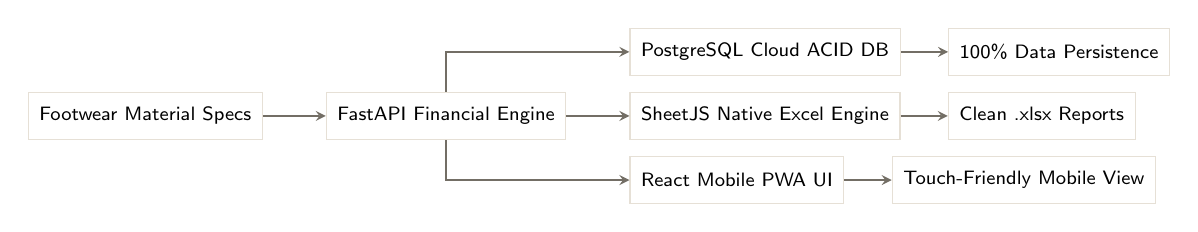
\begin{tikzpicture}[
        node distance = 1.0cm and 0.9cm,
        box/.style = {rectangle, draw=soleborder, fill=white, text centered, font=\scriptsize, minimum height=0.6cm, inner sep=4pt},
        arrow/.style = {->, >=stealth, draw=solegray, line width=0.6pt}
    ]
        \node (specs) [box] {Footwear Material Specs};
        \node (api) [box, right=0.8cm of specs] {FastAPI Financial Engine};
        \node (db) [box, above right=0.2cm and 0.8cm of api] {PostgreSQL Cloud ACID DB};
        \node (sync) [box, right=0.6cm of db] {100\% Data Persistence};
        \node (excel) [box, right=0.8cm of api] {SheetJS Native Excel Engine};
        \node (xlsx) [box, right=0.6cm of excel] {Clean .xlsx Reports};
        \node (pwa) [box, below right=0.2cm and 0.8cm of api] {React Mobile PWA UI};
        \node (mobile) [box, right=0.6cm of pwa] {Touch-Friendly Mobile View};

        \draw [arrow] (specs) -- (api);
        \draw [arrow] (api.north) |- (db.west);
        \draw [arrow] (db) -- (sync);
        \draw [arrow] (api) -- (excel);
        \draw [arrow] (excel) -- (xlsx);
        \draw [arrow] (api.south) |- (pwa.west);
        \draw [arrow] (pwa) -- (mobile);
    \end{tikzpicture}
\end{tcolorbox}

\vspace{4pt}

% --- TWO COLUMN: PROBLEM VS SOLUTION ---
\begin{minipage}[t]{0.485\textwidth}
    {\small \textbf{\color{soleterracotta} 2. Problem Landscape \& Root Causes}}
    \vspace{2pt}
    
    \begin{itemize}[leftmargin=*, itemsep=2.5pt, topsep=1pt]
        \item \footnotesize \textbf{Ephemeral Cloud Data Loss (Render Sleep Cycle):}\\
        On free-tier container hosting, storage is ephemeral. Inactivity after 15 min caused sleep/wake cycles that reset the local SQLite file to the initial Git commit, wiping all user-entered materials.
        
        \item \footnotesize \textbf{Corrupted Excel \& CSV File Exports:}\\
        CSV exports lacked UTF-8 BOM headers, causing Indian Rupee currency symbols to render as corrupted text (\texttt{₹}) and unformatted columns to overflow into \texttt{\#\#\#\#\#\#\#\#} syntax in MS Excel.
        
        \item \footnotesize \textbf{Production Database Test Pollution:}\\
        Automated Pytest suites posted dummy test records (\textit{``Full Grain Bovine\dots''}) directly against the active production database, permanently corrupting the catalog with unwanted fixtures.
        
        \item \footnotesize \textbf{Desktop Navigation \& Mobile Viewport Breakage:}\\
        Legacy views contained unneeded modules (Costing, Sequence, Suppliers) and wide tabular matrices that broke viewport bounds on smartphones with zero responsive touch targets.
    \end{itemize}
\end{minipage}
\hfill
\begin{minipage}[t]{0.485\textwidth}
    {\small \textbf{\color{soleterracotta} 3. Technical Engineering Solutions}}
    \vspace{2pt}
    
    \begin{itemize}[leftmargin=*, itemsep=2.5pt, topsep=1pt]
        \item \footnotesize \textbf{Managed Cloud PostgreSQL Migration:}\\
        Decoupled persistent storage from the container. Integrated \texttt{psycopg2-binary} with SQLAlchemy connection pooling (\texttt{pool\_pre\_ping}, \texttt{pool\_recycle=300}) on Render PostgreSQL for 100\% ACID durability.
        
        \item \footnotesize \textbf{Native In-Browser SheetJS (.xlsx) Engine:}\\
        Replaced broken CSV strings with client-side binary Excel generation (\texttt{xlsx}), applying dynamic column auto-fitting, typed numeric cells, and clean INR (\rupee) formatting.
        
        \item \footnotesize \textbf{Isolated In-Memory Pytest Harness:}\\
        Refactored the test suite using FastAPI dependency overrides and an isolated \texttt{sqlite:///:memory:} StaticPool, ensuring 100\% test isolation without touching production files.
        
        \item \footnotesize \textbf{Claude Design System \& Mobile PWA:}\\
        Redesigned with Anthropic Claude aesthetic (warm parchment \texttt{\#FAF9F5}, terracotta \texttt{\#D97757}), touch targets $\ge 44$px, mobile drawer, and standalone PWA manifest with orange sneaker icons.
    \end{itemize}
\end{minipage}

\vspace{5pt}

% --- SYSTEM ARCHITECTURE MATRIX ---
{\small \textbf{\color{soleterracotta} 4. System Architecture \& Implementation Matrix}}
\vspace{2pt}

\begin{tabularx}{\textwidth}{|l|l|X|}
\hline
\rowcolor{soleterracotta}
\textbf{\color{white} \footnotesize Layer} & 
\textbf{\color{white} \footnotesize Technology} & 
\textbf{\color{white} \footnotesize Key Production Architecture \& Capabilities} \\
\hline
\rowcolor{soleivory}
\footnotesize \textbf{Frontend UI} & \footnotesize React 18 + Vite + Tailwind & 
\footnotesize Claude Design tokens, SheetJS Excel engine, responsive mobile drawer, standalone PWA manifest. \\
\hline
\footnotesize \textbf{Backend API} & \footnotesize FastAPI (Python 3.14) + Uvicorn & 
\footnotesize ASGI asynchronous runtime, Pydantic v2 schemas, automated dual-specification alternative linkage. \\
\hline
\rowcolor{soleivory}
\footnotesize \textbf{Database} & \footnotesize PostgreSQL (Render Cloud) & 
\footnotesize Permanent ACID cloud storage, connection pooling, automated schema creation, zero data loss. \\
\hline
\footnotesize \textbf{Hosting} & \footnotesize Render Web Service & 
\footnotesize Unified full-stack deployment serving static React SPA and FastAPI endpoints under single SSL URL. \\
\hline
\end{tabularx}

\vspace{5pt}

% --- FOOTER ---
{\color{soleborder}\hrule height 0.75pt}
\vspace{2pt}
\begin{center}
    {\tiny \color{solegray} \textbf{Solewise Footwear Intelligence Platform} · Production Live: \href{https://sole-wise.onrender.com}{https://sole-wise.onrender.com} · GitHub: \href{https://github.com/Shree999751/Sole-Wise-}{Shree999751/Sole-Wise-} · Author: Shreyansh Jain}
\end{center}

\end{document}
